\documentclass[11pt,a4paper]{article}
\usepackage[utf8]{inputenc}
\usepackage[T1]{fontenc}
\usepackage{lmodern,amsmath,amssymb,amsthm,mathtools,booktabs,enumitem,microtype}
\usepackage{natbib}
\usepackage{tikz}
\usepackage[margin=1in]{geometry}
\usepackage{xr-hyper}
\usepackage{hyperref}
\externaldocument[GE-]{../../formal/01_law_of_graphic_equalisation_theory_referenced}
\externaldocument[AS-]{../../formal/06_assessing_an_account_of_this_kind}
\newtheorem{proposition}{Proposition}
\title{Is\\\large Relation Without Time, Cause, or Rule}
\author{Matthew Parslow\\Independent Researcher}
\date{\textbf{Draft \texorpdfstring{\textemdash}{---}\ draft-2026-09-02.1}\\[2pt]2 September 2026 \texorpdfstring{\textbullet}{\textperiodcentered}\ document revision 125}
\usepackage{fancyhdr}
\pagestyle{fancy}
\fancyhf{}
\fancyfoot[C]{\thepage}
\fancyfoot[R]{\scriptsize\textsc{draft-2026-09-02.1\,r125}}
\renewcommand{\headrulewidth}{0pt}
\fancypagestyle{plain}{\fancyhf{}\fancyfoot[C]{\thepage}%
  \fancyfoot[R]{\scriptsize\textsc{draft-2026-09-02.1\,r125}}\renewcommand{\headrulewidth}{0pt}}
\begin{document}
\maketitle
\begin{center}
\fbox{\parbox{0.92\textwidth}{\small
\textbf{DRAFT --- draft-2026-09-02.1 r125} (2 September 2026).
This document is under active revision and is circulated for comment, not as a
finished result. Definitions, numbering and claims may change between drafts;
cite the version string above if referring to it. This is the base paper of the
set: \emph{The Law of Graphic Equalisation --- Theory} (referred to below as
Graphic Equalisation) and \emph{Assessing an Account of This Kind} (the
assessment companion) presuppose what is stated here, and those short names are
the only forms used below. Sections marked as falsifiability commitments are the
intended points of attack.}}
\end{center}
\vspace{1em}

\begin{figure}[!ht]
\centering
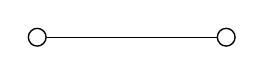
\begin{tikzpicture}
  \draw[line width=0.5pt] (0,0) -- (2.4,0);
  \filldraw[fill=white,draw=black,line width=0.5pt] (0,0) circle (3.2pt);
  \filldraw[fill=white,draw=black,line width=0.5pt] (2.4,0) circle (3.2pt);
\end{tikzpicture}
\caption{Is.}
\label{fig:is}
\end{figure}

\begin{abstract}
One claim, made without machinery. To be is to stand in relation and to cohere in it, and nothing
further is required for there to be anything at all --- no sequence, no cause, no rule about what may
follow what, \emph{and no observer}. Observation is not primitive here, and it is not derived
here either --- it is \emph{absent}, and the companions derive it, in accounts that
posit what deriving it takes. So what merely stands in relation cannot observe. And where nothing contains it, it cannot be
observed either, only modelled. Nothing in this account waits on anything looking. The
companion accounts presuppose this claim and say so; this one states what they presuppose. The claim is short. This paper is not, and on its own accounting need not
be: what is being asked for is the sentence, and the rest is the case for it.
\end{abstract}

\section{The claim}\label{sec:claim}
\emph{What is, is.} That is the whole of it, and everything below is an attempt to say what the sentence
commits to and what it does not.

One thing it does not commit to should be said before anything else, because the machinery below is
routinely read as committing to its opposite. \emph{Observation is not primitive, and it is not derived here.} It is
\emph{not present at all}: making a distinction is an act, acts need transformation and a grammar of
what may follow, and this account has neither --- so the deriving happens in the companions, at the
point where they pay for those, and what this paper describes cannot observe --- and, there being nothing to contain it, cannot be
observed either, only modelled (Proposition~\ref{prop:one-way}). An observer is a late and expensive
thing, and nothing here waits on one.

To be \emph{something} rather than nothing at all is to be distinguishable, and to be distinguishable is
to stand apart from something. \emph{Distinction is relation.} There is no third option in which a thing
is determinate and stands in no relation whatever.

\emph{That sentence is a commitment and not a result, and it is the one place to disagree.} It holds
that a determinate something must be distinguishable, and that distinguishability is irreducibly
relational. Positions denying it are available and are not silly: a thing might be determinate through
an intrinsic character, a primitive thisness, or its own numerical identity, with no second thing
anywhere. Nothing below derives this away. What is offered against it is a price rather than a
refutation --- such a character has to be \emph{posited}, and it is a posit no relation registers,
which is the one thing the norm in Section~\ref{sec:method} charges for. A reader willing to pay it
should stop at this line, because everything after it is downstream. \emph{The disagreement belongs
here and not several pages later.}

Three claims come apart, and the paper is easier to attack once they are separated. \emph{One:}
determinacy is relational --- the commitment just made. \emph{Two:} time, cause, rule and an observer
are not entailed by it, which is what the removals below establish. \emph{Three:} removal against a
shortest-sufficient standard is a reasonable way to audit what an account carries, which is
methodological and neither of the first two. The second and third can fail without touching the
first, and the first can be rejected on its own.

\begin{proposition}[To be is to be related]\label{prop:is}
Anything that exists as a determinate something stands in at least one relation. Contrapositively:
where no relation holds, there is no distinction, and where there is no distinction there is no
determinate something --- not one that cannot be told apart from nothing, but no second thing there to
be told apart.
\end{proposition}

\emph{Figure~\ref{fig:is} is the claim.} There is nothing else to draw, and the omissions are the content: no names, no types, no arrowhead, no distinction between the marks beyond where they sit, and \emph{no border} --- a border is a boundary, a boundary belongs to whatever draws it, and at this level there is nothing to draw one, nor anything for the figure to be inside. It demonstrates what it states rather than illustrating it.

What makes the \emph{marks} two is their position on the page, which the page supplies; what makes the \emph{relata} two is the relation between them, which Section~\ref{sec:graph} argues and nothing in the drawing shows. A reader taking the left mark as first reads a direction off the paper. The page is the container the drawing cannot escape and declines to assert. All of that is supplied. What is not is that there is a difference here at all.

\emph{What is} is the subject, and nothing else is. Where a sentence here looks as though it quantifies
over what does not exist, the failing item is a description and not a thing --- the care Proposition~\ref{prop:is}
takes in saying \emph{no second thing there to be told apart}.

\subsection*{What the words carry}
Four words do the work, and each is used in one sense throughout. They are given here rather than
assembled as they arrive, because a reader who lets any of them drift between an ontological, a
logical and an informational reading will find the propositions below proving more than they do.

\emph{Relatum.} An end of a relation, and nothing else. Not a substance, not a bearer of intrinsic
properties, not an object carrying an identity condition supplied from somewhere --- there is nowhere
here for one to be supplied from. What makes two relata two is the subject of
Section~\ref{sec:one-not-enough} and is not assumed here.

\emph{Relation.} A tie with ends. Not an ordered pair drawn from a domain fixed in advance, which is
the textbook construction and is a \emph{construction}; why that order is unavailable at this level is
given in Section~\ref{sec:prior}. It carries no type, no direction and no weight, each of those being
supplied by whatever describes it rather than found in it.

\emph{Distinction.} Two ends failing to collapse into one. This is the identification made above, and
it is where disagreement with this paper belongs.

\emph{Coherence.} A relation coheres when its ends are distinct. That is stated as a condition and
not derived from anything, and saying so is the honest version: it is the structural exclusion of the
two zero-distance cases --- nothing related, and a thing related only to itself --- and the exclusion
is what does the work everywhere below. It is not an epistemic measure, presupposes no observer, and
requires no informational state, language, frame or evaluator, none of which exist at this level and
all of which the account would have to buy. The informational reading --- that a relation carries a
fact about one end given the other that was not already had --- \emph{agrees} with it here, and is how
the companions carry the criterion forward once there are frames to measure against. The agreement runs
in that direction only. \emph{The base condition is structural; the informational criterion is what it
becomes once there is something to measure with}, and a reader who takes the second for the ground of
the first will look for an evaluator this level cannot supply and correctly fail to find one.

One consequence of the last of the four is worth stating rather than leaving to be inferred. A criterion for
existing that \emph{needed} a frame would index existing to frames, which is the reading this account
refuses everywhere else; so the floor has to be the structural one. \emph{What carries nothing carries
nothing for anything.}

\emph{The verbs.} Those four are nouns and the same care is owed to what the paper does with them,
because the hazard here is not a word but a tense. \emph{The exposition is sequential because an
argument is written and read in time. Nothing in that order is an order within the base described.}
\emph{Removal}, \emph{derivation}, \emph{addition}, \emph{arrival}, \emph{survival} and \emph{later}
name relations among descriptions and commitments in the metatheory; they do not name stages through
which what is passes. There is no before-the-graph, no graph-after-removal, and no graph that exists
and then acquires an edge. Where the prose below runs in sequence --- and it does, throughout, because
prose has no other way to run --- the sequence belongs to the account and not to its subject. This is
not a promise to avoid such verbs, which would make the paper unreadable. It is the instruction for
reading them.

\section{Remove, and see what breaks}\label{sec:method}
A claim of this shape is worth nothing if it arrives by assertion, and the difference between an account
and a pronouncement is whether there is a procedure behind it that someone else can run. There is one here, and it is short.

\emph{One thing about it has to be said before the norms, because a reader will otherwise supply the
wrong object.} What the procedure removes are \emph{candidate posits in an account} --- time, cause,
rule, substance, an observer --- and not edges from a graph. \emph{The graph is what the procedure
arrives at, not what it operates on}, and nothing below is a claim about what breaks when a structure
is cut. The vocabulary that follows is accordingly the vocabulary of assessing accounts, and it is used
here and nowhere else in this paper.

\emph{That is one instance of a distinction the whole paper rests on, and it is cheaper to state once
than to rely on.} The base has no logic, no inference, no norms and no rules: that is the claim.
Stating the claim uses all four. There is no contradiction in this, and there would be one in
pretending otherwise --- an argument is conducted in a metalanguage, and what a metalanguage requires
is not thereby part of what it describes. Inference, the exclusion of incoherent descriptions, the
preference for the shorter account, the removal tests, the judgement that coverage held: every one of
these belongs to the assessing and none to the assessed. \emph{A description of a level with no rules
is not itself at that level.} The reader is owed this because without it the denial of rules reads as
self-undermining, which it is not; and where this paper slips and attributes a metalinguistic resource
to the base, that is a defect and should be reported as one rather than absorbed.

\emph{Ask at maximum scope.} The question is put to everything at once rather than to a domain, because
a shortest sufficient account of one domain tells you about that domain and a shortest sufficient
account of all of it tells you what is common to all of it. The scope is what does the work: the more
that must be accounted for, the more the structure peculiar to any part washes out and the more only
what is shared survives.

\emph{Prefer the shortest account that suffices.} Between two accounts covering the same ground, the one
carrying less structure is preferred, and this is the ordinary discipline of minimum description length
rather than anything invented here. Applied at maximum scope it has a direction: keep removing until
removing costs coverage.

It is also why \emph{shortest} needs a frame, and that is not a defect: description length is defined
only against a vocabulary, which is what Graphic Equalisation's Axiom~\ref{GE-ax:no-view} insists on,
and what its Remark~\ref{GE-rem:mdl-ontic} accepts in the form that the constant is the frame.

\emph{Remove, and see what breaks.} This is the operation and it is the only one. Take a candidate ---
time, cause, rule, substance, an observer, a global clock --- and put the account without it. If what
was accounted for is still accounted for, the candidate was not required and it goes. If coverage is
lost, it stays, and the loss shows what it was doing. Each removal is a test whose outcome is determinate in one
direction and not in the other, and the asymmetry is this: a
\emph{successful} removal settles the matter, since an account that stands without the candidate is
exhibited and can be inspected, while a \emph{failed} one records only that nobody has yet seen how,
and stays open to a reader who does. That is what makes the procedure repeatable rather than a matter
of taste.

Run that far enough and it stops in one place. Time can go: nothing in the claim requires sequence.
Cause can go: relation is not production. Rule can go: nothing needs to be permitted or forbidden for
things to stand as they stand. Substance can go: nothing here bears properties, and a relatum is an
end. A global clock can go with time. Relation cannot go, because removing it removes distinction, and removing
distinction removes the possibility of there being determinate somethings for the account to be about at
all. \emph{The claim is not asserted here. It is what survived} --- survived, that is, given the
identification made in Section~\ref{sec:claim}. Relation is what cannot go \emph{because} distinction
was granted to be relational; the removals show that nothing else is needed alongside it. They do not
establish the identification, and nothing in this paper does.

\emph{A removal must be named and restorable.} This is the discipline that separates the method from
mere simplification, and it is the one place the procedure can be abused. Every account reached this way
is an idealisation, and an idealisation is just a frame --- which is no defence on its own, since
everything is one. What makes a frame cheap to hold rather than expensive is whether what it removed is
written down and can be put back. The rock is what this claim looks like \emph{from outside}, at the grain at which it is a
rock --- the embedded case of Section~\ref{sec:one-way}; the case this paper posits has no outside and
no rock. That its atoms move and it weathers at other grains belongs on the same page, so the removed
structure is recoverable and the idealisation costs little. \emph{The spherical cow is not objectionable
for being spherical.} It is objectionable when nobody writes down that it was made spherical, and the result is then applied
to a cow.

Which this paper owes of itself, and this is the place. \emph{It was made spherical by removing frames.}
Nothing described here is individuated by anything, and everything real is: individuation is performed
by a container, that container is individuated by its own, and there is no last one. So the base set out
here is not a thing anybody meets, and it cannot be reached by stripping either, the stripping not
terminating. \emph{Nor is it an earlier stage of anything.} What is described is an idealised
ontological floor and not a temporally prior physical state --- there is no time here for it to be
prior in, and a reader supplying a cosmological reading is restoring the sequence this section exists
to remove. Written down, then: what was removed is frames, acts, and any grammar of what may follow,
and where it goes back is the companions, which restore all three and pay for them in a ledger.

The kind of removal matters and is part of writing it down. A spherical cow is \emph{false} of a cow.
Nothing here is false of anything real --- every actual thing does stand in relation and does cohere,
and goes on doing both once its frames are put back. This paper is true of everything and complete about
nothing, which is the only shape an account at this scope could have. \emph{It is an idealisation by
subtraction and not by distortion}, and the subtraction is the whole of what makes it short.

This paper also has to come first: a base that already assumed
frames would be assuming the thing the companions exist to pay for, and their pages would then read as
commitment rather than as derivation. Starting from an object with no instances is the cost of starting
anywhere at all.

The norm is not this programme's invention. It is Occam's razor, and \citet{rissanen1978} is where it
stops being a preference --- \emph{do not introduce structure that buys no additional distinction} ---
since \emph{simpler} settles nothing until someone says simpler in what units. \citet{shannon1948}
supplies that measure and \emph{not} the norm, containing no model selection, so citing the two
together for the norm borrows a name that did not make the claim. What is added here is only the scope at which it is applied.

Removal establishes that nothing \emph{tried} was required, which is not the same as nothing being
required. The result is only as good as the candidate list, so that list should be stated rather than
implied: time, causation, substance or intrinsic nature, an observer, a privileged frame or global
clock, admissibility, and --- less obviously --- any axiom restricting where a distinction may be made
from.

The last of those is worth naming, because it is the one kept by habit: a rule that every distinction
is made in some frame governs frames, and there are none here to govern. It arrives with the machinery
it constrains, which is where Graphic Equalisation states it, as its Axiom~\ref{GE-ax:no-view}, and it
is not required for anything this paper says.

Removing it does not remove every commitment about distinction, and the two are easily run together.
\emph{Removed}: any rule about where a distinction may be made \emph{from}. \emph{Retained, and
load-bearing}: the denial of a privileged characterisation, which forces the graph
(Section~\ref{sec:graph}) and is this paper's one prohibition; and that a distinction is a relation, which is the identification the whole
claim turns on, and a commitment rather than a discovery. A reader who holds that a thing can be
determinate without standing apart from anything rejects this paper at that sentence and needs to go no
further --- which is where the disagreement should be, rather than several pages downstream.

Every entry on that list is a \emph{posit}, something an account might assert exists, and a list of one
kind is short by a whole category. A commitment can also arrive as a \emph{word}: vocabulary carrying
something it does not declare, which no reader stops on because it does not present as a claim at all.
\emph{Type} is the worked case --- calling a graph typed asserts that kinds are part of what is there,
and Graphic Equalisation settles in its Remark~\ref{GE-rem:types-forced} that they are not,
distinctness being forced where sameness is supplied.
\emph{Substance} is the worse case: already on the list, it can return inside the very sentence that
claims to have decomposed it away, which is what Graphic Equalisation's Remark~\ref{GE-rem:one-substance}
refuses in those terms. The operation is the same one; only the candidates are new. Remove the
word and see whether any claim alters: vocabulary doing no work goes silently, and vocabulary carrying
a smuggled commitment takes a claim with it.

Anyone who thinks something else belongs at the base is invited to add it and run the same procedure,
and that is the form disagreement with this paper should take.

\subsection*{One operation, applied to what came bundled}
The operation is stated above as removing posited structure --- time, cause, rule ---
but its more productive target is different, and is the same operation pointed the other way.

Almost every claim worth taking at maximum scope is one that some field already accepts, and accepts
with a restriction attached. Relations are basic \emph{in this formalism}. There is no privileged
observer \emph{in mechanics}. The shortest description is preferred \emph{for this class of model}.
The restriction is generally not a discovered property of the subject; it is the restriction that
constitutes the field, and it travelled with the claim because within a field there was never an
occasion to separate them. So the move is to take the claim seriously and decline the restriction ---
which is not a new procedure but \emph{remove, and see what breaks} applied to an inherited limit
rather than to a posited entity, with the same asymmetric outcome and the same requirement that the
removal be named and restorable.

Two things follow. The
first is that results reached this way look simultaneously trivial and consequential, and are both:
trivial because nothing was added and the claim was already granted, consequential because the
discarded restriction was doing work that nobody had audited, having never been separable from the
subject inside the field that held it. The limit that keeps this from being a recipe is stated next.

The second is a limit, and it is severe. Most restrictions are load-bearing --- they are attached
because removing them breaks something, and taking a claim past its restriction usually produces
nonsense rather than generality. The operation is cheap to run and returns nothing on almost every
attempt --- a rate this paper commits to in Section~\ref{sec:falsifiability} --- and the ones that
return something are worth reporting for that reason and not because
the operation is powerful. Nothing here is a recipe for producing results by taking things literally.
It is a cheap test, run often, with a low yield, and a signal on firing that is clear about \emph{that}
something did not break while saying nothing about whether what survived is worth having.

\section{One is not enough}\label{sec:one-not-enough}
A single relatum is a valid candidate for examination and this paper does not get to forbid it. One
may formulate it, draw it, name it and investigate it --- all of that from a frame outside the case,
which is where the formulating happens and is exactly the metatheoretic position
Section~\ref{sec:method} sets apart. \emph{At the base it contains no relation from which a distinction
could be constituted.} It has no second end and no boundary, so there is nothing there that a
distinction could be made across --- not even a distinction from the absence of a second relatum.
\emph{And the absence is not temporal.} It is not that a second relatum has not yet appeared, nor that
one is somewhere pending: there is no relation present at all, and no sense in which the case is
waiting on anything. Reading it as a not-yet imports the sequence Section~\ref{sec:not-claimed} denies
and turns a structural verdict into an episode.

So the verdict is not that the one-node case is meaningless or that it cannot be drawn. It is that on
the commitment of Section~\ref{sec:claim} it does not constitute a determinate existent: it supplies
no relation by which its relatum could be distinct from anything. \emph{One relatum does not cohere},
in the sense the definition above gives --- its ends, such as they are, are not distinct. It does not
sit at the bottom of the hierarchy of existing things, and does not stand outside it awaiting entry. And it earns its place here
by being the candidate that shows why the minimum must contain a relation with \emph{distinct} ends
rather than merely a relation: not one node, but two relata in a non-self relation.

The empty case is the other end and is cleaner. Nothing at all stands in no relation, has no parts to be
in tension, and admits no failure of fit --- it is complete in the only sense available to it. That is
why the empty set is the only perfect thing and why perfection is not something an existent can have:
\emph{to exist is to be imperfect}, because to exist is to be related, and to be related is to be
partial with respect to what one is related to.

The two ends meet, and where they meet is the point. The failed case yields nothing because the
relation has no distance to cross; the empty case yields nothing because there is nothing to cross to.
Reading either off gives the same result --- nothing --- and so does a third: everything at once, read
from outside, has nothing left over to stand in relation to it, and gives nothing too. \emph{That is the
correct reading of the old claim that everything and nothing come to the same}, and it is a claim about
two \emph{readings}, never about two things. The version that drops the qualifier asserts the identity
from a standpoint, and there is no standpoint at which it holds. From anywhere at all --- which is the
only place anything is --- everything is emphatically not nothing. Between the two zeros is where the
distinctions live, and everything this paper is about lies there.

\section{Coherence, and what fails to cohere}\label{sec:cohere}
\begin{proposition}[To exist is to cohere]\label{prop:cohere}
A relation suffices only where it \emph{coheres}: where its ends are distinct. Neither degenerate case
is a thing that fails the condition: where no relation holds there is nothing to cohere, and where the
only relation is to oneself the ends are not two. In both, what fails is the \emph{description}, which
picks out nothing. Relation is necessary; coherence is what makes it sufficient.
\end{proposition}

Proposition~\ref{prop:cohere} is not a refinement offered for tidiness.
Proposition~\ref{prop:is}, read alone, is satisfied by a thing related only to \emph{itself} --- the
letter met and the point defeated, since the two ends of such a relation do not come apart. That is why
the prose above says \emph{distinguishable} where Proposition~\ref{prop:is} says \emph{stands in at
least one relation}: the two come apart there, and the prose was the accurate one. \emph{Things that do
not cohere are not there to fail.}

\emph{The measured rendering is the one the companions use, and it is not the ground of the condition.}
Once there is something to measure against, to cohere is for a relation to \emph{carry} something --- a
fact about one end given the other that was not already had --- which makes the criterion a quantity
rather than a condition met or not met by inspection, and sorts every case by that one measure. Nothing
related: no relation, nothing carried. Related only to itself: a relation, nothing carried. Two things
related: something carried, and the only one of the three that is anything. That rendering
\emph{agrees} with the structural condition everywhere both apply, and the agreement runs in that
direction only: the base condition is structural, and the measured criterion is what it becomes once
there are frames to measure with.

\emph{Two further readings sort the same three cases the same way, and neither grounds the
condition.} Consistency asks whether things can be held together; information asks whether holding one
tells you about another. Read either way the cases sort identically, and a self-relation lands at the
end where holding is trivial rather than the end where it is impossible --- which is why its failure is
emptiness and not prohibition. The agreement is worth having, being what lets the companions carry the
criterion forward as a measured quantity. It is not an argument for the condition, and this paper does
not offer it as one. The verdict is settled without a frame, for the reason the definition of
\emph{coherence} above gives, so the degenerate cases are degenerate absolutely.

It is tempting to conclude that rules are needed after all --- that something must \emph{enforce}
coherence, and enforcing is what rules do. The temptation comes from hearing the question as \emph{what
can be created}, and the question here is \emph{what can exist}. Creating needs an agent, an act, and a
grammar governing the act, and this paper has none of the three. \emph{Nothing excludes the incoherent
cases, and nothing needs to}, not existing being no outcome that has to be brought about. What coheres,
coheres; what does not is not there; and no rule stands between the two doing work.

The smallest case shows the two coming apart. A graph of one node can be \emph{created} --- drawn,
named, saved to a file --- and does not thereby exist in this paper's sense, one relatum standing apart
from nothing. Labelling it does not rescue it, a label being supplied by whatever draws it rather than a
relation the node has, which is the point Figure~\ref{fig:is} makes about its two marks. So creation is
neither necessary nor sufficient for existence here, and the companions --- about worlds in which things
happen, and therefore about making --- are where rules belong, as is something already picked out
ceasing to cohere.

\section{One direction only}\label{sec:one-way}
A consequence of the restraint deserves its own statement, because it is what makes the claim's subject
matter peculiar. \emph{What merely is cannot observe.} Whether it can be \emph{observed} turns on whether anything
contains it; in the case posited here nothing does, and it can only be \emph{modelled}.

To observe is to make a distinction, and making one is an act --- something is done, and afterwards the
observer holds what it did not hold before. That requires transformation and some grammar of what may
follow what, and this paper has neither. So what is described here does nothing at all, and observing is
among the things it does not do.

Two cases have to be separated here, and running them together is an error. \emph{Where the base is
embedded} --- a level inside a world that has containers --- it can be the object of observation without
difficulty, and a rock is what that looks like from outside: met, related to, distinguished by something
that does have the machinery.

\emph{The scenario posited here is the other case.} The base is embedded in nothing, because it is
everything there is. \emph{So there is no container to instantiate a boundary} --- and instantiating is
what a container does, as this section has just said --- \emph{so there is nothing to observe it, and no
observation occurs}. To say it \emph{can be} observed grants an outside the scenario does not contain,
which is the free import of a relation, in the section whose whole work is to refuse exactly that.

\emph{What remains available is modelling.} The model is a metatheoretic representation \emph{of} the base --- of
it, and not merely of the modeller's own notes, since a representation of nothing in particular would
be arbitrary rather than non-observational. What it is not is an observation performed inside the
scenario: the representing relation belongs to the modeller's frame and adds no edge, no boundary and
no observer to what is described. \emph{One can model what one cannot touch}, and touching is what is
unavailable here. \emph{Which is what this paper does.} It does not observe what it describes. It models
it, from a frame that is not in the scenario at all --- and saying so is not a confession but a
statement of the only access there is.

But there is no corresponding inside. \emph{There is no view from anywhere} --- not a narrow
view, not a limited one, none.

The reason is not that framehood needs rules --- it does not, and Graphic Equalisation's
Remark~\ref{GE-rem:only-g} is explicit that a structure with no rules of its own is still a frame,
because \emph{individuation is performed by the container and not by the thing}. A boundary belongs to the frame that draws it, so what a rule-less
structure lacks is not framehood but the capacity to individuate anything itself. It is also why an
\emph{empty} frame is impossible rather than merely unattested: an edge needs relata, so where there is
nothing there is nothing to demarcate.

What the base lacks is the drawing: it is a frame in every account that models it --- this one
included --- and contains none, there being nothing in it to instantiate one.

What is missing is \emph{making}. A view is not had by standing in a relation; it is had by a frame
that \emph{makes} a distinction, and making is doing, and doing is what this level does not have ---
that is precisely what the companions add when they admit that things happen. So the familiar claim,
that every view is had from somewhere by someone positioned, presupposes there are views and asks where
they are from. Here there are none to ask about: \emph{no view from nowhere, and no view from anywhere
either}, not for want of a place to view from but for want of anything doing the viewing.

An axiom restricting where a distinction may be \emph{made} from therefore cannot be stated at this
level, let alone assumed --- because it governs an act, and there are no acts here; it arrives with the
machinery that performs them --- which is also why there are no frames at this level to govern, since
instantiating a boundary is one. The other half of that axiom is a different matter and is retained:
denying that any characterisation is privileged says nothing about acts or frames, and it is what makes
the graph a result rather than a preference.

\begin{proposition}[Observation is one-directional at the base]\label{prop:one-way}
What stands in relation without transformation or grammar cannot observe. Where a container exists it
can be observed, and is then always the object of a distinction and never the maker of one. Where none
exists --- the case posited here --- \emph{it can be modelled and not observed}, modelling requiring no
relation to its object.
\end{proposition}

\section{Which is to say: a graph}\label{sec:graph}
The claim has a name, and refusing to use it would be coy. Relata standing in relations are nodes
standing in edges. \emph{Everything is a graph} is the companions' thesis. What is established here is
narrower and is all they need: \emph{the bare untyped graph is the least ontology this account may
retain}, stated in the only form that requires nothing to state it.

\emph{Which graph} has to be said, because the word carries a construction that is not meant, and a
reader supplying the textbook one will find the claim presupposing most of what it denies. At the floor
meant here, \emph{graph} names no labels, values, types, directions, weights, metrics or external
embedding. It names relata and a relation between them, and nothing else.

A node is an \emph{end} of a relation, recoverable from the relation rather than prior to it --- which
is the definition given above and not a second one. It is why the two nodes of $K_2$ are nodes although
neither is where anything meets. That is the reverse of the order mathematics needs, for reasons
Section~\ref{sec:prior} gives in full and which are not a quibble about notation.

Three things that follow are worth settling here rather than leaving to be reconstructed.

\emph{The minimum is not an arbitrary graph with an edge in it.} It is two nodes joined by one edge.
A lone node fails for the reason Section~\ref{sec:one-not-enough} gives, and a self-loop fails for the
reason Proposition~\ref{prop:cohere} gives: each supplies a structure without supplying a nontrivial
distinction, and neither is a small existent but a failed one. So the smallest coherent instance is
$K_2$, and the condition on a base graph is not that its edge set is non-empty but that some edge has
distinct ends.

\emph{The two ends are distinct without being qualitatively different, and this is the sharpest place
to press the argument.} In $K_2$ the nodes have identical structural profiles: swapping them changes
nothing, and there is no label, intrinsic mark or property to tell them apart --- by construction,
since the floor has none to offer. What makes them two is the irreflexivity of the relation between
them. They are \emph{weakly discernible}: distinct as the two ends of a relation that nothing bears to
itself, which is discernibility without a discerning property and is exactly the notion the identity of
indiscernibles was found to need \citep{black1952,saunders2003}. That literature reached it for
physics, where the case is fermions rather than a base graph; the notion is the same one and is not
this paper's invention. A reader who rejects weak discernibility rejects the second node here, and
lands back at the commitment in Section~\ref{sec:claim} --- which is the correct place for the
objection to arrive.

\emph{The set-theoretic apparatus is the metatheory's encoding and not additional furniture.} Sets,
ordered and unordered pairs, membership and the incidence construction are how an account writes a
graph down; the ontology asserted is nodes and an edge. This is the object-language distinction of
Section~\ref{sec:method} applied at the point where it is most easily lost, and it is the same
distinction that keeps ``no rules at the base'' consistent with the formal rules used to state the
claim.

That step needs one thing, without which the graph is a choice of notation
among richer ones and the obvious question --- why not a manifold, why not something with an order or a
metric built in? --- has no answer. One answer suggests itself, is not available, and should be refused first, because it is the one this
paper would otherwise be read as giving. \emph{A richer intrinsic form could be asserted only from a
standpoint at which the extra structure is visible, and no such standpoint is available} --- from which
nothing follows about whether the form is there. What can be asserted and what is the case are
different questions, and an argument running from the first to the second is the slide from an
epistemic limit to an ontic absence. The prohibition below constrains what may be \emph{claimed}. It
does not by itself empty the world of whatever no claim could reach, and this paper does not get to
have it both ways.

What does the work is the measure, and it is already on the table. Structure making no difference to
any relation buys no additional distinction, and the norm of Section~\ref{sec:method} --- Rissanen's,
not this paper's --- removes precisely that. A metric earns its place wherever some relation registers
it; where none does, it is carried and never read, and carrying it is the silent cost the whole method
exists to charge for. So the account declines it. \emph{That is a claim about the account and not a
proof about the world}, and the difference is not cosmetic: someone willing to posit an intrinsic form
that no relation registers may have one, and pays a posit for something no relation could ever report
back. This paper's method is the refusal to pay on those terms. It is weaker than a demonstration of
impossibility, and it is what is available.

In the metatheory, where there is something to measure with, the denial is sharper as a measure, since
the phrase invites the wrong
picture. A view is informative in proportion to the relation between viewer and viewed --- what the one
tells you about the other is what a view delivers. A view from nowhere stands in no relation to what it
views, so it delivers \emph{nothing}: not a partial view or a distorted one, but zero. So it is not the
complete view we are being denied; it is the empty one, and a standpoint that adds nothing to what it
sees receives nothing from it either. Read off from nowhere is read off at no information, which is not
reading anything off --- and that is why what survives is relation and nothing above it.

Which means this paper is not adding an axiom here, and Graphic Equalisation's numbering of it as
Axiom~\ref{GE-ax:no-view} should be read accordingly. To be is to stand in relation; a relation is what carries
information; so a standpoint in no relation to what it views carries nothing about it. The denial
follows from the claim and the measure, and posits nothing further. It is stated all the same, and
stated as a prohibition, because what it denies is imported for free --- a reader supplies the
standpoint without deciding to, so a consequence nobody would otherwise draw has to be put where the
import happens. So what survives every standpoint \emph{as a claim} is the bare relational
minimum, and what this account retains is therefore a graph. That is what the discipline leaves; it is
not what the world is shown to lack.

This is Graphic Equalisation's Axiom~\ref{GE-ax:no-view} doing a job at this level, and only half of it: the frame-governing
half has nothing to govern here, for the reason Section~\ref{sec:one-way} gives. What is used is the
denial of a privileged characterisation, and it is used as a constraint on claims rather than as the
ontological premise the previous paragraph declined to make of it.

It also gives this paper the one prohibition it has. Why it must be a
prohibition rather than a removal is also why Graphic Equalisation numbers it as it does, for the
reason its Remark~\ref{GE-rem:why-minus-one} gives. Everything else here
is removal: take a candidate away and see whether the account still stands. This one cannot be removed that way, because \emph{it is not in the
text to be taken out}.

A reader does not arrive neutral on whether there is a view from nowhere --- they
arrive already using one, having read a claim as being about how things are rather than how things are
from somewhere, which is the default and costs nothing to adopt. What is imported for free returns
unless it is refused explicitly, and an axiom that cancels a default has to be stated before the
counting starts. Hence a prohibition, and hence its number. A \emph{claim} that some structure has an
intrinsic form readable from no standpoint would violate it; a world is not the kind of thing that
can.

The question this paper asks is the dumbest one available: \emph{what is there?} A child can ask it and
nothing prevents anyone answering. It is also the largest, because an answer to it constrains every
answer to anything else, and because there is nowhere further back to stand.

The form of this paper follows from that. It builds \emph{no machinery}, deliberately: no
transformation, no grammar, no economics --- none of the apparatus a reader could dispute
\emph{instead of} disputing the claim. That is not the same as offering nothing else to disagree with. What follows below is a method, a reading of how
formalisms move under compression, and an accounting of what derivation costs; each is separable from
the claim and each can be rejected on its own. The form that survives is narrower: no \emph{structure is
posited} here that could absorb an objection meant for the claim, so a reader who rejects the claim
cannot be answered by adjusting a mechanism, because there is none to adjust.

The objection that arrives immediately can be answered in a line. \emph{Everything can be
represented as a graph, so the claim is empty} --- yes to the first clause, and this is not a claim
about representability. Nodes and edges are cheap; what is asserted is that there is \emph{nothing
else}, that relata and relations exhaust what there is, and that time and cause and rule in
particular are not among the furniture. What would bear on it is a demonstration that this world has
time or cause in its floor --- \emph{which is empirical and not modal}, so imagining a world that does
costs nothing and settles nothing.

Finding one would bound the account rather than refute it, in the way a later theory bounds an earlier:
the claim would hold of worlds without such a floor and this would not be one of them.

\section{A consequence with a track record}\label{sec:track-record}
The claim fixes what compression is aiming at, and that turns out to be checkable in a way the claim
itself is not.

If what there is, is relata standing in relations, then the shortest sufficient description of anything
is stated \emph{in terms of} relata and relations. The qualification is doing real work. Without it the
claim becomes that a description shorter than its subject's structure has lost something --- which is a
picture theory, and worse, contradicts the accounting of Section~\ref{sec:method}. Minimum description length charges for a generator, not for what unrolling it produces:
the shortest sufficient description of the complete graph on a million vertices is a phrase naming the
relation and the count, not five hundred billion enumerated pairs, and a description isomorphic to its
subject is very often the expensive one. So the claim cannot be that the shortest description
\emph{enumerates} relata and relations.

What it can be, and is, is a claim about the vocabulary the generator has to be written in. ``The
complete graph on a million vertices'' is a short generator whose terms are a relation type, an arity
and a count; it is about relata and relations without listing any. \emph{The arity and the count are
the generator's parameters and not values borne by anything at the floor}, which is worth saying here
rather than leaving to Section~\ref{sec:falsifiability} to concede: they belong to the description
doing the generating, in the metatheory, and the thing generated carries no labels at all. A reader who
reads them as furniture has found the objection that section takes up, and has found it one section
early. The prediction is therefore that
formalisms under compression converge on \emph{primitives} that are relata and relations, not on
descriptions the size of their subjects. \emph{The ideal information shape is a graph} in that sense
--- what the terms denote is fixed by what is being described, while how briefly they can be combined
is not. So a field pushing its own formalism toward minimum description should \emph{move toward}
graph form, and it should do so without anyone intending it. \emph{That is the older claim that
information is what everything is made of} \citep{wheeler1990,bateson1972}, stated for everything rather
than for physics.

That is a prediction about the history of formalisms rather than about the world, and it appears to
hold. \emph{The cases named next are illustration and not the evidence for it}, no entry having been
checked here against the movement the prediction is about, which is the discriminator this section
closes on; the case the fourth commitment rests on is the one set out at length below, where the
movement can be dated. Where fields have settled is the visible part: physics reaching for spin
networks, tensor networks and causal sets; chemistry settling on the
molecular graph; linguistics on dependency structure; computing on data structures that are graphs and on a categorical foundation in which the morphisms
are primitive and the objects recoverable from their identities --- which is the vertices-from-edges
order this paper needs, reached there for reasons of its own; neuroscience on the connectome; biology on
phylogenies and interaction networks. None of these was adopted because anybody held the thesis of this
paper. Each was adopted because it was the cheapest thing that still accounted for the subject.

One case is set out rather than listed, being the oldest, the longest kept,
and it is usually described as an invention. \emph{Double-entry bookkeeping is not an invention. It is
a compression.} A transfer has two sides, and the record that keeps both of them names two accounts and the movement
between them --- relata and a relation and nothing else. It should be said at once that this
is not a minimality claim, because \citeauthor{ellerman2014} refutes the obvious one: a single-sided
system using signed numbers records the same information, and given the same opening equation and the
same transactions the two end in the same place. What single-sided recording loses is the trial
balance, and that is the whole of the difference worth having here. Nobody derived it from a thesis about what exists.

The history is what makes it a case rather than an analogy. \citet{pacioli1494} is usually credited
with the system, and what he wrote was a description: the \emph{Particularis de Computis et Scripturis},
a treatise inside a mathematics textbook, setting out a method already in use among Venetian merchants.
The practice is older than the account of it by roughly two centuries --- \citet{lee1977} reads the
Farolfi ledger of 1299--1300 as full double entry --- so the system was found in use and then written
down, which is the order a compression arrives in and not the order an invention does. And it has been
kept for five centuries, in the formalism the field teaches and computes with, which is what the
commitment below actually asks for.

The counterweight belongs here too, because the history is contested in a way that bears on the
claim. \citet{yamey1949} argued against the then-standard view that double entry was adopted for
rational profit calculation, holding that early merchants did not use it that way. What Yamey found
is a \emph{smaller} purpose rather than none --- tracking debtor and creditor relations, custody,
and agency accountability --- and \citet{sangster2016} names it more precisely: the system gave a
clear picture of every debtor and creditor \emph{together with the means to check that the entries
between them were complete and accurate}. So Yamey does not license the inference that the method
was adopted with no theory of what it was for. It was adopted for something, and the something was
checking --- which forecloses any argument here from nobody having designed the technique for
anything, and means the error-detection property below was not a lucky side effect but what the
thing was built to do, and why it was kept.

And it earns the case rather than illustrating it, because of what the practice detects. A ledger that
does not balance is not a rule violation but a \emph{residual} --- something recorded that does not
cohere with the rest --- and the trial balance is a coherence check, which is why the technique catches
errors at all. A convention that did not match the two-sidedness of what it records would have no such
property, so the survival of the technique is evidence about the subject and not only about the
bookkeepers.

That reading has a mathematical statement and it is not this paper's.
\citet{ellerman1985,ellerman2014} shows that double entry implicitly uses the \emph{group of
differences} over pairs of unsigned numbers --- the T-account is the pair --- so a transaction is a
difference and the two entries are its two components rather than one record written twice. Balance is
then the group identity, and an unbalanced ledger is a residual in the exact sense, which is where the
error-detecting property comes from. The dating is the part that bears on the claim here: the structure was in use long before anyone had the mathematics to say what it was, and the interval is given exactly below.

And \citet{aryagraph2000} reach the relata-and-relations reading without the thesis, characterising
the consistent transaction vectors by a \emph{directed graph representation of the accounting system},
without which recovering transactions from statements \citep{arya2000} becomes intractable as accounts
multiply.

The discriminator matters and is easy to lose. \emph{The prediction is about movement, not about
drawability.} That a field's subject matter can be drawn as a graph shows nothing, since graphs are
expressive and almost anything can be. What would count is a field that compressed its formalism and
moved \emph{away} from graph form --- toward a primitive that is not a relatum or a relation and cannot
be reduced to them --- and that is what the second commitment below asks for.

\section{What is not claimed}\label{sec:not-claimed}
The claim above is smaller than it may appear, and the restraint is the point.

\emph{No time.} Nothing here requires sequence. Relations hold; they do not happen. There is no earlier
and no later in this paper, and no order in which anything is arrived at.

\emph{No cause.} Nothing here makes anything else be. Relation is not production, and the account has no
resources with which to say that one relatum brings about another.

\emph{No rule.} Nothing here forbids anything or licenses anything. There is no admissibility, nothing
that may or may not follow, and therefore nothing that could be violated. The coherence criterion does
not smuggle one back, because \emph{nothing enforces it}: what coheres is not permitted to, it simply
does.

Those are not oversights and they are not deferred out of modesty. \emph{They cost extra} --- and the third is what \emph{making} anything requires, which is why a paper
about what can exist rather than what can be created does none of it. A world
in which things also \emph{happen} requires transformation and a grammar of what may follow what, and
that is what the companion accounts introduce and pay for. This paper is what remains when they are
removed, and it is offered as evidence that they are separable rather than constitutive.

\section{What the companions add}\label{sec:companions}
The companion accounts presuppose this claim and posit past it what a world in which things
\emph{happen} costs, which is not required for there to be anything.

\emph{The relation between them and this paper is one of dependence rather than temporal genealogy.}
A changing graph presupposes the bare relational condition, while the bare relational graph does not
presuppose transformation, grammar or observation. \emph{The asymmetry is ontological}: it concerns
what each condition requires, and requirement is not a sequence in which one state becomes another. So
the bare graph comes first \emph{in requirement} and need not be an earlier state at all --- nothing
here asserts that a world passed through a static graph before becoming a changing one. The ordering of
the accounts mirrors that requirement; it does not stand in for it, and it is not what the precedence
consists in.

\emph{And they begin with a graph that is not an axiom of theirs.} This paper does not assume that
everything is a graph. It establishes that, given relational determinacy and the
no-unpaid-structure discipline, \emph{the bare untyped graph is the least ontology this account may
retain}. The qualification is not a hedge appended to a stronger claim; it is the whole of what
Section~\ref{sec:graph} licenses. So the companions inherit graphhood as a \emph{result within that
discipline} rather than as an independent postulate, and their axioms concern \emph{change} in that
graph rather than the graph's existence. What is established nowhere here is that nonrelational
structure registering in no relation is impossible. Someone may posit it. What this account says of it
is that it is unwarranted, which is a different word from unavailable and is the only one earned.
Graphic Equalisation's own ledger, its Table~\ref{GE-tab:ledger}, carries the admission and two
postulates named there --- a realisation operator and a destroy\slash preserve distinction --- with its
Axiom~\ref{GE-ax:no-view} a discipline against
importing unpaid assumptions in that paper and a commitment that can fail in the groundings.

Three things are posited past it and none of them is free: transformation, so that something does the
happening; an economics, so that a change has a price; and realisation, so that what is admissible
becomes what occurs. \emph{The case that each is cheap is made in the companions and not here}, which
is where it belongs --- this section says what is taken on, not what it costs to take.

So what the companions add to this paper is the admission that things happen --- transformation ---
and the two postulates its ledger names, realisation and the destroy\slash preserve distinction that is
the economics, and past those the bets they state as hypotheses rather than as commitments. What
follows unpacks those commitments; none of it adds to what exists.

The strong form of the statement is therefore false and the useful form survives: the base is small,
what is added to it is enumerable, and anything in the companions that is an independent posit
uncounted by that enumeration is a defect in their economy. That standard has been applied to them; the companions do not exempt themselves from it, and the
record of its application is in the assessment companion's Section~\ref{AS-sec:turned} rather than
here. Their not exempting themselves is the
prohibition above applied to the writing: an account stating its rules from outside its own scope would
be speaking from the standpoint this paper denies, and that standpoint is imported freely enough that
refusing it once is not enough.

\section{Prior positions}\label{sec:prior}
None of this is new and it should not be dressed as though it were. The neighbours are easy to name.
That relations are prior to, or on a level with, their relata is the ontic structural realist position
\citep{ladymanross2007,esfeld2004}; that a thing is nothing over and above what it stands in is older
and starker \citep{nagarjuna1995}; and the bundle tradition reaches a neighbouring conclusion by a
different route \citep{dcwilliams1953}.

The relation to them is not the usual one, and the difference can be stated exactly rather than as a
matter of emphasis. \emph{Each of those accounts supposes a particular \textbf{type} of relation where
the argument only requires that there be one.} Ontic structural realism is a thesis about physics --- about what our best theories say the world is
made of --- and its restriction is that \emph{domain} rather than any particular edge. The structure it
argues for is physical structure, and its live disputes are about objects, relations, modality and
identity; characterising it as an observer edge would be a misreading, and this paper does not need
one. The perspective literature is the case where an edge genuinely is fixed, viewing being
constitutive there. Neither is mistaken about the structure. One is restricted to a domain and the
other to an edge, and the removal applies to each in its own way.

The removal is immediate and is the method's own. Where an edge is fixed, take it out and put any
other in its place --- a gravitational one, a chemical bond, mere adjacency, one part of a rock against
another --- and everything the structural claim needs is still there. Two relata and a relation between
them do not care which relation it is, so what is treated as constitutive is a \emph{choice of edge
type}, salient in the domain it was written for and doing no work in the claim itself. Where a domain
is fixed instead, the removal is the other one: declining an inherited restriction, asking of
everything what physics licensed about physical structure, and seeing whether anything breaks. In both
cases what survives is the claim this paper makes, and in neither case is that claim new.

The same over-specification is visible in the two fields that own this vocabulary, which are the ones a
reader will expect to have settled the matter. Information theory defines
its quantities over a source and a channel: there is something sending, something receiving, and a
distribution over what might have been sent. Those roles are formal and need nobody to occupy them --- reading a source as an
observer is an error the theory does not commit, and it is worth not committing it here either. What is
fixed is nonetheless a \emph{distinguished pair of roles}, which is why entropy is a property of a
source-and-receiver arrangement rather than of a thing. The restriction is of the same kind and arrived
for the same reason: the field's problems were communication problems, and had two ends by
construction. And
graph theory, in its standard presentation, takes a vertex set first and defines edges as pairs drawn
from it --- which builds in the priority of relata over relations before any question about that
priority has been asked. Neither field is careless. Each fixed an edge type or an order of construction
because its own problems required one.

Which yields the deflationary version of this whole paper. \emph{If everything is a graph, then the
minimum structure required to be a graph is the least structure this account may retain.} That structure
is not something this paper discovers: it has been written down in every textbook of the subject for a
century, as relata and relations and nothing else. What is being done here is not deriving it but
\emph{taking it seriously} --- reading a definition that was built as a formalism as though it were an
answer to the largest question, and then checking that nothing else has to be added. The removals above
are that check. That is the entire contribution, and it is smaller than it sounds while being, if the
claim holds, sufficient.

One qualification even there. The textbook definition takes
a vertex set as given and edges as pairs over it, which makes relata prior --- and it does so for a good
reason. \emph{Graph theory's objects do not need to exist.} They are built, and building takes an order:
you must have the vertices in hand before you can say which pairs of them are edges. The priority is a
feature of \emph{construction}, and construction is what mathematics does.

Nothing here is constructed. What exists was not assembled in an order, and there is no stage at which
the relata were available and the relations not yet drawn. So the priority does not merely go unneeded
in this paper --- it is \emph{unavailable}, and for a reason already established: an order of
construction is a sequence, and there is no time here for one to run in. A definition that builds cannot
be read as a description of something that was never built without carrying its scaffolding across.

Graph theory is not over-specified for its
own purposes; it is exactly specified for constructing objects. What does not transfer is the
scaffolding, and noticing that it is scaffolding is most of the work of taking the definition
seriously.

That is also why the closest neighbour is the one furthest from physics. \citet{nagarjuna1995} makes the
claim in a form that does not require an observer edge --- nothing needs to be looking, measuring or
theorising for a thing to be nothing over and above what it stands in --- which is the property the
others lack, and which only became the discriminating one once the edge type was seen to be removable.
That reading is contested, and the stronger form --- that there is no observer edge anywhere in the
account --- is not one the secondary literature licenses: conceptual or nominal dependence
is standardly the third and strongest of the dependence relations at issue, and on that reading the
carving is ours. What the comparison needs is only the weaker claim, that the position is
\emph{statable} without the edge, which both readings allow.

There remains the fact that this is simple enough to state in a sentence and appears not to have been
stated, which invites the reaction that it must therefore be either trivial or wrong. The account has its own explanation
for that pairing and it is in the assessment companion's Section~\ref{AS-sec:objection}, so a short one
will do here, and the short one
is structural rather than a remark about incentives. \emph{People do not study everything. They study
something.} A field is constituted by its restriction --- what it attends to and what it sets aside ---
and a field with no restriction is not a field. So the question this paper asks, which has to be put at
maximum scope or it is not the same question, belongs to no discipline: there is no subject matter of
which it is the subject matter, and no method calibrated for it, because every method is calibrated to
a something.

That is why the general form goes unwritten while every local version gets written well.

And the mechanism has a worked case in this paper already, which makes
the explanation checkable instead of merely available. The gap between double entry being in daily
use and the group of differences being written down is about three and a half centuries --- Pacioli in
1494 to Hamilton's ordered couples of 1837, on \citeauthor{ellerman2014}'s own attribution --- on top of the two centuries
between the practice and Pacioli's description of it. That is not a hard construction: it is how the
integers are built from the naturals.

The reason it went unwritten is \emph{not} that nobody looked. Mathematicians did look --- \citeauthor{ellerman2014} names De Morgan in 1869 and Cayley,
who published a pamphlet on double-entry bookkeeping in 1894 --- and did not make the ordered-pairs
identification. So the case is weaker than a clean two-restriction gap and is still a case: a trivial
structure in continuous use by thousands of people, examined by capable people from the other side, went
unformalised anyway. \citeauthor{ellerman2014} adds the part that bears on the mechanism, which is that
placing the identification took him three decades to publish in an accounting journal. The restriction
is real; what it obstructed was the crossing rather than the looking.

The parallel is in the sociology and not in the content, and the difference matters. What double entry
says is not what this paper says. What the case establishes is that \emph{a thing can be simple, in
constant use, and unwritten for centuries, for no reason except that no field owned it} --- which is the
mechanism this section claims, evidenced somewhere it can be dated. Whether this paper's claim is
another instance of it is not something the case decides, and a reader who thinks the sentence is
trivial and wrong rather than trivial and unwritten is disagreeing with the claim, which is the right
place to disagree with it. It also
explains, without needing a separate reason, why such statements tend to arrive from someone crossing
between domains: crossing is what asking at maximum scope looks like from inside an arrangement where
every position is a restricted one.

The claim of absence is held loosely, and more loosely than the rest of the paper. Nobody could be
confident of having searched exhaustively. It is an invitation: if this has been written down as a claim about what
exists, rather than as a formalism or as a thesis within one field, the right response to this paper is
the reference.

What is contributed is accordingly not the thesis but its \emph{position}: that it is enough on its own;
that time, cause, rule, an observer, and any axiom about where distinctions may be made from are not
required for it; and that an account of how things change can be built on top without folding any of
them back in. The companion papers are that account, and what they presuppose is this one.

\section{Falsifiability}\label{sec:falsifiability}
Four commitments, in the order of the three claims separated in Section~\ref{sec:claim} and then the
prediction. The first is what the paper claims; the second is that time, cause, rule and an observer
are separable from it; the third is a claim the paper makes about its own method; the fourth is what
the claim predicts, and is the easiest to test once \emph{compression pressure} is operationalised, and
the one for which a proxy is offered meanwhile.

\emph{They are not the same kind of claim, and calling all four falsifiable flattens a difference that
matters.} The first is \emph{conceptual}, and is assessed the way claims of its kind are assessed: by
whether it coheres, what it costs, what it forces elsewhere, and whether a rival buys more with less.
No measurement settles it, and presenting it as though one might would be a borrowed credential. The
second is settled by whether an account of change can be built without folding a removed candidate back
in, which is a matter of construction rather than of measurement. The third and fourth are ordinary
empirical claims --- about a method's yield, and about the history of formalisms --- and they carry
what risk is carried here. \emph{The groundings carry the rest.}
Where the companions put the claim to work in physics, in cosmology and in mind, it stops being a
discipline on an account and becomes a commitment that can fail against observation; that is where the
exposure sits, and it is deliberate that it sits there rather than here. Saying so is not a retreat
from falsifiability. It is declining to claim a kind of testability this paper does not have, while
naming the two places it does.

Each commitment below is marked \textsc{[shape]} or \textsc{[detail]}. A \textsc{[detail]} failing is
a revision: the account survives with that mechanism replaced. A \textsc{[shape]} failing costs
\emph{range} rather than a mechanism, because what fails is something the substrate is claimed to
require or to permit --- so the account does not hold where it claimed to, which is the more serious
of the two and is still a boundary rather than an annihilation.

\begin{enumerate}[leftmargin=*]
\item \textsc{[shape]}~\textbf{To be is to be related.} A claim about this world and not about every
possible one. Met by an intelligible counterexample --- a determinate something for which standing in
any relation at all is \emph{coherently} deniable --- or by a rival account at lower cost and equal
coverage. An unrelated existent merely \emph{asserted} is not one: the attempt decoheres, and that
outcome is checkable, for the reasons given below the list. Unknown or unmeasured relations are not the
case at issue either, that being the ordinary condition of most things; what is asked for is something
of which the claim that it stands in any relation at all is false. The burden is entirely on that side:
no enumeration establishes the claim, since the domain does not terminate, and one instance would bound
it.

\item \textsc{[shape]}~\textbf{Time, cause, rule and an observer are separable.} What the removals of
Section~\ref{sec:method} establish, and what the companions are offered as evidence for. Fails if the
account of change built on this one could not be constructed without folding one of them back into the
base --- in which case the restraint claimed in Section~\ref{sec:not-claimed} would be a fiction and
this paper would be an incomplete statement of the base rather than a minimal one. This counts against
the paper without falsifying the first commitment, which is why it is a separate item. It is also
bounded, not failed, by a demonstration that this world has time or cause in its floor
(Section~\ref{sec:graph}): the claim would then hold of worlds without such a floor and this would not
be one of them.

\item \textsc{[detail]}~\textbf{The method's yield is low.} The claim that the operation of declining an
inherited restriction returns nothing on almost every attempt, which this paper leans on --- it is what
makes a rare result evidence of a discipline rather than of a machine for producing results. It is also
a base rate over attempts nobody recorded: no ledger of the failures was kept, so the rate is
reconstructed rather than recorded, which is a defect and is stated as one. It fails if a record of such
attempts, kept prospectively rather than reconstructed, shows the operation succeeding often; and this
paper owes that record before the claim should be granted. Marked \textsc{[detail]} because it is
methodological and can fail without touching the first commitment.

\item \textsc{[detail]}~\textbf{Compression moves toward graph form.} A consequence of the first, and a
prediction about the history of formalisms rather than about the world, which is why it is marked as it
is. What is at issue is the \emph{bearer of the field's distinctions}: whether
what a field individuates and quantifies over under compression pressure is relata and relations, with
the rest carried as labels on them, or whether the individuated thing is something else. Fails if a
field's primitive bearer of distinction stops being relata-and-relations --- if the field adopts under
compression pressure a primitive that is neither and \emph{keeps} it, carrying it in the formalism the
field teaches and computes with rather than in a reduction nobody uses. \emph{The commitment awaits an
operationalisation of \emph{compression pressure} and is not yet testable without one}; the proxy
offered meanwhile is the formalism the field's standard textbook teaches, read across successive
editions.

The wording is chosen rather than found, and the reason should be visible. A commitment about whether a
formalism carries \emph{only} relata and relations would be about nothing, since none does and none is
likely to: \emph{the complete graph on a million vertices} keeps an arity and a count, and neither is a
relatum or a relation; every confirming case above keeps something similar --- amplitudes, irrep
labels, branch lengths, edge weights --- each taught and computed with. Those are the generator's
parameters and the labels riding on what is individuated, which is why the commitment is worded about
the bearer of distinction and not about the inventory. What is asked is retention and not
irreducibility, because graphs are expressive enough that almost any candidate can be argued to reduce,
and a test whose confirming door is shut by that fact must not have its refuting door bolted by it too.
Expressiveness is not at issue in the other direction either: that a subject \emph{can} be drawn as a
graph is no evidence, and only the direction of movement under compression counts.
\end{enumerate}

\subsection*{Two objections to the first commitment}
Two objections arrive at the first commitment, and both have to be met, because between them they say
what kind of claim the proposition is.

\emph{The first} runs: the account holds that the description of an unrelated existent \emph{picks out
nothing}, so the falsifying case is one in which there is no fact to report, and a falsifier nothing
could answer to is not a falsifier. The first half is granted. The conclusion is not, because it assumes
that a falsifier which cannot be \emph{coherently} met is thereby not a falsifier, and the distinction
those two run together is the one this whole account is about.

\emph{Neither bare verdict is available here, and reaching for one is where this goes wrong.} Calling
the commitment falsifiable, or calling it unfalsifiable, both import a frame in which a counterexample
would be a \emph{coherent} state of affairs --- describable, then looked for. The reader supplies that
frame at no cost, having no reason to suspect it is doing work, and it is the whole of the difficulty:
the distinction this commitment turns on sits \emph{below} the grain at which falsifiability is
ordinarily argued, so a reader is not disagreeing about it but not resolving it. Said in full, then, and without the word that does not fit
it: the commitment admits a determinate attempt with a determinate outcome, and that outcome cannot be
a coherent counterexample. Calling this falsifiability borrows the credential the opening of this
section declined; calling it unfalsifiability reports only that no measurement settles it, which was
never in dispute. \emph{The challenge this claim takes is conceptual} --- an intelligible
counterexample, or a rival account with lower cost at equal or better coverage. Drop the qualification
and the sentence reverts to whichever verdict the reader already had.

A claim with no content has no attemptable counterexample at all:
put one to a vocabulary and you get another expression in the vocabulary, which is not a failure of
anything. Put one to this claim and the attempt has a determinate outcome --- it decoheres, in the exact
sense of Graphic Equalisation's Proposition~\ref{GE-prop:decoherence-one}, returning nothing with the
whole of the frame as residual. That outcome is
checkable, and it is distinguishable by inspection from the vocabulary case: \emph{I tried and got
nothing back} is a different result from \emph{there was nothing to try}.

What the objection has found
is not that the claim risks nothing. It is that the claim is at maximum scope, so the only thing that
could refute it is the one thing the claim says cannot be assembled --- and a question whose refutation
would have to be incoherent is the most a question of this shape can be, not the least.

\emph{The second} is the one a reader reaches for first. It runs: exhibiting a counterexample means
observing it, observing relates it to the observer, so anything offered as unrelated is related by the
act of being offered, and the falsifier cannot be met.

That slides from \emph{relation} to \emph{observation}, and the two are not the same. \emph{Observation
is not required for existence.} The tree falls in the empty forest and stands in relation throughout ---
to the ground it strikes, to the air it moves, to its own fibres as they part --- and not one of those
relations waits on anybody looking. Observation is a \emph{kind} of relation, and a late and expensive
one, since it requires a frame with the machinery to make a distinction; relation is the general case
and requires nothing.

So the claim here is not that to be is to be perceived, which is a different thesis with a different
name and is not held. What is claimed is that to be is to be \emph{related}, and the falsifier asks for
something standing in no relation whatever --- not for something unobserved, of which there is a great
deal. That makes the commitment harder to meet rather than easier, since a candidate cannot be rescued
by pointing out that it is now related to whoever produced it: the question is whether it stood in any
relation at all, and the fallen tree settles that without an observer anywhere.

Proposition~\ref{prop:one-way} survives this unchanged. What merely is still cannot observe. It simply
does not follow that it needs to be observed in order to be.

\begin{thebibliography}{99}
\itemsep=2pt

\bibitem[Arya et~al.(2000a)]{arya2000}
Anil Arya, John C. Fellingham, Jonathan C. Glover, Douglas A. Schroeder, and Gilbert Strang.
\newblock Inferring transactions from financial statements.
\newblock \emph{Contemporary Accounting Research}, 17(3):366--385, 2000.

\bibitem[Arya et~al.(2000b)]{aryagraph2000}
Anil Arya, John C. Fellingham, and Douglas A. Schroeder.
\newblock Estimating transactions given balance sheets and an income statement.
\newblock \emph{Issues in Accounting Education}, 15(3):393--411, 2000.

\bibitem[Bateson(1972)]{bateson1972}
Gregory Bateson.
\newblock \emph{Steps to an Ecology of Mind}.
\newblock Chandler, San Francisco, 1972.

\bibitem[Black(1952)]{black1952}
Max Black.
\newblock The identity of indiscernibles.
\newblock \emph{Mind}, 61(242):153--164, 1952.

\bibitem[Ellerman(1985)]{ellerman1985}
David P. Ellerman.
\newblock The mathematics of double entry bookkeeping.
\newblock \emph{Mathematics Magazine}, 58(4):226--233, 1985.

\bibitem[Ellerman(2014)]{ellerman2014}
David Ellerman.
\newblock On double-entry bookkeeping: the mathematical treatment.
\newblock \emph{Accounting Education}, 23(5):483--501, 2014.

\bibitem[Esfeld(2004)]{esfeld2004}
Michael Esfeld.
\newblock Quantum entanglement and a metaphysics of relations.
\newblock \emph{Studies in History and Philosophy of Modern Physics}, 35(4):601--617, 2004.

\bibitem[Ladyman and Ross(2007)]{ladymanross2007}
James Ladyman and Don Ross.
\newblock \emph{Every Thing Must Go: Metaphysics Naturalized}.
\newblock Oxford University Press, Oxford, 2007.

\bibitem[Lee(1977)]{lee1977}
Geoffrey A. Lee.
\newblock The coming of age of double entry: the Giovanni Farolfi ledger of 1299--1300.
\newblock \emph{Accounting Historians Journal}, 4(2):79--96, 1977.

\bibitem[N\=ag\=arjuna(1995)]{nagarjuna1995}
N\=ag\=arjuna.
\newblock \emph{The Fundamental Wisdom of the Middle Way: N\=ag\=arjuna's M\=ulamadhyamakak\=arik\=a}.
\newblock Translated by Jay L. Garfield. Oxford University Press, New York, 1995.

\bibitem[Pacioli(1494)]{pacioli1494}
Luca Pacioli.
\newblock \emph{Summa de Arithmetica, Geometria, Proportioni et Proportionalit\`a}.
\newblock Venice, 1494.
\newblock The bookkeeping treatise is the \emph{Particularis de Computis et Scripturis}.

\bibitem[Rissanen(1978)]{rissanen1978}
Jorma Rissanen.
\newblock Modeling by shortest data description.
\newblock \emph{Automatica}, 14:465--471, 1978.

\bibitem[Sangster(2016)]{sangster2016}
Alan Sangster.
\newblock The genesis of double entry bookkeeping.
\newblock \emph{The Accounting Review}, 91(1):299--315, 2016.
\newblock Published online 2015.

\bibitem[Saunders(2003)]{saunders2003}
Simon Saunders.
\newblock Physics and Leibniz's principles.
\newblock In Katherine Brading and Elena Castellani, editors, \emph{Symmetries in Physics:
Philosophical Reflections}, pages 289--307. Cambridge University Press, Cambridge, 2003.

\bibitem[Shannon(1948)]{shannon1948}
Claude E. Shannon.
\newblock A mathematical theory of communication.
\newblock \emph{Bell System Technical Journal}, 27:379--423, 623--656, 1948.

\bibitem[Wheeler(1990)]{wheeler1990}
John~A. Wheeler.
\newblock Information, physics, quantum: The search for links.
\newblock In Wojciech~H. Zurek, editor, \emph{Complexity, Entropy, and the Physics of Information},
pages 3--28. Addison-Wesley, Redwood City, 1990.

\bibitem[Williams(1953)]{dcwilliams1953}
Donald C. Williams.
\newblock On the elements of being: I.
\newblock \emph{The Review of Metaphysics}, 7(1):3--18, 1953.

\bibitem[Yamey(1949)]{yamey1949}
Basil S. Yamey.
\newblock Scientific bookkeeping and the rise of capitalism.
\newblock \emph{The Economic History Review}, 1(2/3):99--113, 1949.

\end{thebibliography}
\end{document}
